\item \begin{theorem}{(7)} DRAM是capacitor,比較便宜且體積小,但速度較慢;SRAM是latch。Cache用SRAM。
\end{theorem}

\item \begin{theorem}{(25, 27, 38, 48, 124)} Cache:\begin{itemize}
        \item Write:\begin{itemize}
            \item Write-through:寫入cache和memory。
            \item Write-buffer:寫入cache和buffer且CPU繼續執行,當buffer滿時,CPU須等到buffer有空位。
            \item Write-back:只寫入cache。
            \item Write allocate:從memory拉進cache,在cache中修改。
            \item Write around (No write allocate):不拉進cache,只在memory中修改。
            \item 通常write-though配write around,write-back配write allocate。
        \end{itemize}
        \item Split cache通常有較差hit ratio,提升bandwidth,但不提升speed。
        \item 增加associativity:降低miss rate,增加hit time。
        \item L1 cache:注重減少hit time;L2 cache:注重減少miss ratio。
        \item Cache miss is handled by cache controller.
    \end{itemize}
\end{theorem}

\item \begin{theorem}{(53)} \begin{equation}
        L_nGMR  = \PI_{i = 1}^{n}L_iLMR   
    \end{equation} 
\end{theorem}

\item \begin{theorem}{(54)} Average Memory Access Time (AMAT):\begin{equation}
        AMAT = hit \ time + Miss \ rate \times Miss \ penalty   
    \end{equation} Using multilevel cache and non-blocking cache both reduce miss penalty.
\end{theorem}

\item \begin{theorem}{(61, 66, 71, 78, 86, 88, 124)} Virtual memory:\begin{itemize}
        \item fully mapping因為怕存取HD太慢,write-back,large page size。
        \item 減少page table size:\begin{itemize}
            \item 使用limit register限制分頁大小。
            \item 兩張page tables和兩個分開的limit registers。
            \item Inverted page table:儲存virtual page no.和physical page no.,並使用hash function,因此virtual page table size和physical page table一樣即可。
            \item Multilevel page table:但address translation太複雜。
            \item 允許page table也被分頁,但必須避免無止盡的page fault。
        \end{itemize}
        \item reference bit:決定victim page。
        \item TLB:\begin{itemize}
            \item 存tag和physical page no.。
            \item TLB一般使用fully associative的TLB,lower miss rate,且size較小,lower cost,且一般使用random置換。
        \end{itemize}
        \item Page fault is signaled by hardware.
        \item TLB miss result in TLB exception.
        \item \quad\quad \begin{itemize}
            \item Physically indexed and physically tagged:將所有virtual address translate physical address再access。
            \item Virtually indexed and virtually tagged:使用virtual address access cache,only translate if going to memory,但若有一page被share,在cache有多個objects,造成aliasing。
            \item Virtually indexed and physically tagged:Always translate before going to cache. 解決virtual addressed cache aliasing問題。
        \end{itemize}
        \begin{figure}[H]
            \centering
            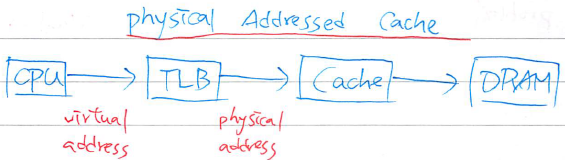
\includegraphics[scale=0.7]{img/phy-phy-cache.png}
            \caption{Physical adressed cache.}
        \end{figure}
        \begin{figure}[H]
            \centering
            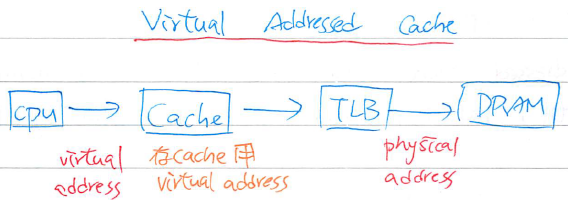
\includegraphics[scale=0.7]{img/vir-vir-cache.png}
            \caption{Virtual addressed cache.}
        \end{figure}
        \begin{figure}[H]
            \centering
            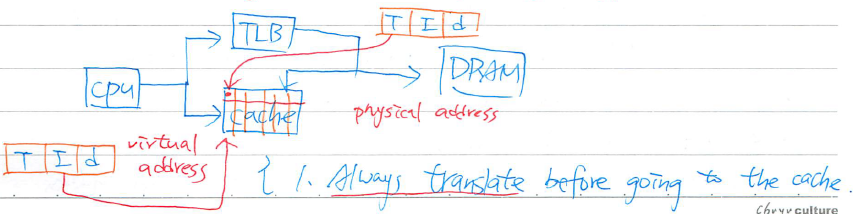
\includegraphics[scale=0.7]{img/vir-phy-cache.png}
            \caption{Virtually indexed and physically tagged cache.}
        \end{figure}
        \item Non-blocking cache:Cache miss時,CPU繼續access cache,通常用在superscalar的out of order execution,用來隱藏cache miss time。
    \end{itemize}
\end{theorem}

